\documentclass{article}
\usepackage[utf8]{inputenc}
\usepackage[spanish]{babel}
\usepackage{xcolor}
\usepackage{wrapfig}
\usepackage{amsmath}
\usepackage{amsfonts}
\usepackage{amssymb}
\usepackage{graphicx}
\usepackage{hyperref}
\usepackage{lipsum}
\usepackage{multicol}


\date{\today}
\author{Nicolas Cardona Ramirez}


\begin{document}
	
	\title{\textcolor{violet}{Curso de MatLab}}
	\maketitle
	
	\section{Episodio 10: Formato de Salida}
	
	\subsection{\textcolor{blue}{Notación Científica}}
	
	Se utiliza para escribir número con un valor muy grande o muy pequeño. En MatLab se utiliza:
	
	\begin{itemize}
		\item  6.022e23
	\end{itemize}

	\subsection{\textcolor{blue}{Cambiar formato de Números}}
	
	\begin{itemize}
	
	\item Para utilizar 14 cifras decimales se utiliza \textcolor{green}{format long}
	
	\item Para utiliza 2 cifras decimales se utiliza
	\textcolor{green}{format bank} y se aproxima la última cifra decimal
	
	\item El formato por defecto con 4 cifras decimales es \textcolor{green}{format short}
	\item El \textcolor{green}{format +} despliega solo los signos positivos y negativos dentro de una matriz
	
	\item El \textcolor{green}{format rat} despliega los números como números racionales, es decir, como fracciones
	
	\item Para cambiar la forma de la notación científica se utiliza los comandos anteriores más la letra e; \textcolor{green}{format short e}
	
	\end{itemize}
	
	
	\section{Episodio 11: Funciones en MatLab}




	\subsection{\textcolor{blue}{Funciones Internas}}
	
	Las funciones internas más utilizadas son:
	
	\begin{itemize}
		\item Para usar raíz cuadrada se utiliza \textcolor{green}{sqrt()} y puede ser una matriz o un vector
		\item La función \textcolor{green}{rem(a,b)} calcula el residuo de dos números
		\item La función \textcolor{green}{[x,y] = size(d)} calcula el tamaño de una matriz o de un vector y tiene dos parámetros de salida donde \colorbox{orange}{x} es el número de filas y \colorbox{orange}{y}
		
	\end{itemize}
	
	\subsection{\textcolor{blue}{Funciones anidadas}}

	Para realizar una función anidada se utiliza \textcolor{green}{sqrt(sin(x))}

	\section{Episodio 12: Funciones Matemáticas}
	
	Las funciones matemáticas esenciales son:
	
	\begin{itemize}
		\item \textcolor{red}{abs()}: absoluto
		\item \textcolor{red}{sqrt()}: Raíz cuadrada
		\item \textcolor{red}{nthroot (x,n)}: Enésima raíz real de x
		\item \textcolor{red}{sign()}: Regresa el signo del número
		\item \textcolor{red}{rem(x,y)}: Residuo de x/y
		\item \textcolor{red}{log()}: Calcula el logaritmo natural de x
		\item \textcolor{red}{log10()}: Calcula el logaritmo base 10 de x
	\end{itemize}

	\subsection{\textcolor{blue}{Funciones de Redondeo}}
	
	Las funciones de redondeo son:
	
	\begin{itemize}
		\item \textcolor{red}{round(b)}: Redondea al número entero más cercano
		\item \textcolor{red}{fix(b)}: Redondea al entero más cercano a cero
		\item \textcolor{red}{floor(b)}: Redondea al entero mas cercano hacia el infinito negativo
		\item \textcolor{red}{ceil(b)}:Redondea hacia el entero más cercano hacia el infinito positivo
	\end{itemize}

	\begin{figure}[h!]
		\centering
		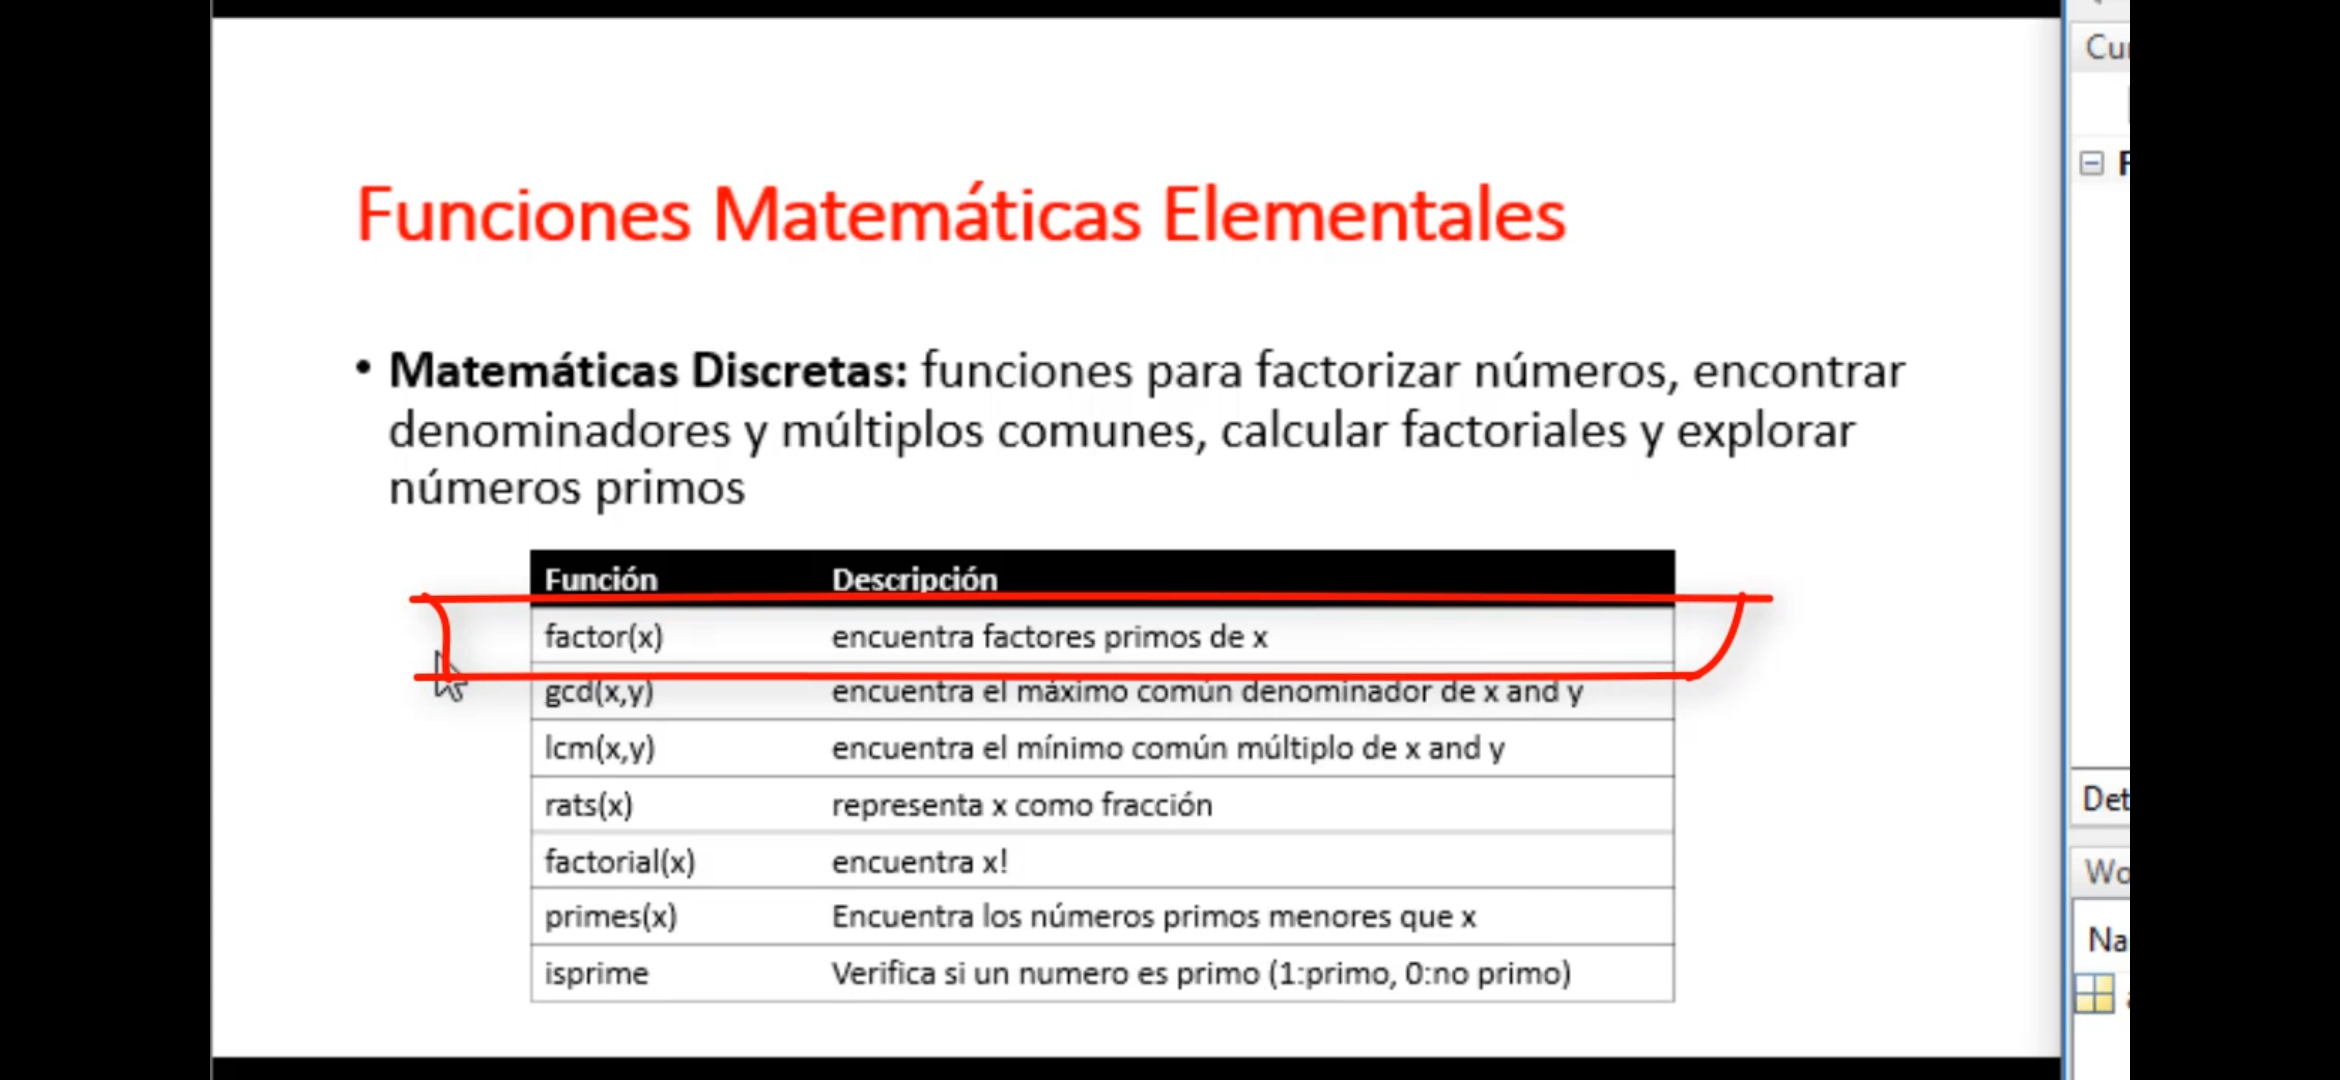
\includegraphics[width = 100mm]{imagenes/math_discre}
		\caption{Funciones matemáticas discretas}
		\label{discretas}
	\end{figure}

	\section{Episodio 13: Funciones Trigonométricas}

	Los ángulos deben de estar en radianes
	
	\begin{equation}
	grados = radianes \left(\frac{180}{\pi}\right)
	\end{equation}
	
	\begin{equation}
	radianes = grados \left(\frac{\pi}{180}\right)
	\end{equation}
	
	Las funciones trigonométricas estandares son:
	\begin{multicols}{2}
	\begin{itemize}
		\item sin(x) con x en radianes
		\item cos(x) con x en radianes
		\item tan(x) con x en radianes
		\item csc(x) con x en radianes
		\item sec(x) con x en radianes
		\item cot(x) con x en radianes
		\item sind(x) con x en grados
		\item cosd(x) con x en grados
		\item tand(x) con x en grados
		\item cscd(x) con x en grados
		\item secd(x) con x en grados
		\item cotd(x) con x en grados
	\end{itemize}
	\end{multicols}

	\subsection{\textcolor{blue}{Funciones Trigonométricas Inversas}}

		Las funciones trigonométricas inversas son:
	\begin{multicols}{2}
		\begin{itemize}
			\item asin(x) con x en radianes
			\item acos(x) con x en radianes
			\item atan(x) con x en radianes
			\item acsc(x) con x en radianes
			\item asec(x) con x en radianes
			\item acot(x) con x en radianes
			\item asind(x) con x en grados
			\item acosd(x) con x en grados
			\item atand(x) con x en grados
			\item acscd(x) con x en grados
			\item asecd(x) con x en grados
			\item acotd(x) con x en grados
		\end{itemize}
	\end{multicols}

	\subsection{\textcolor{blue}{Funciones Trigonométricas Hiperbólicas}}

	\begin{multicols}{2}
	\begin{itemize}
		\item sinh(x) con x en radianes
		\item cosh(x) con x en radianes
		\item tanh(x) con x en radianes
		\item csch(x) con x en radianes
		\item sech(x) con x en radianes
		\item coth(x) con x en radianes
	\end{itemize}
\end{multicols}

	\section{Episodio 14: Análisis de Datos en MatLab}
	
	\begin{itemize}
		
	\item Para encontrar el \colorbox{orange}{máximo} de una matriz entrega el resultado del máximo por cada columna o un vector se utiliza la función \textcolor{green}{max()} y para guardar su posición se utiliza \textcolor{green}{[a,b] = max()} donde \colorbox{orange}{a} es el máximo y \colorbox{orange}{b} es su posición.

	\item Para encontrar el \colorbox{orange}{mínimo} se utiliza la funcinó \textcolor{green}{min()}
	
	\item Para \colorbox{orange}{trasponer} una matriz se utiliza el nombre de la matriz mas comilla; \textcolor{green}{max(y')}
	
	\item Para hacer una \colorbox{orange}{sumatoria} de los elementos de un vector o matriz se utiliza el comando \textcolor{green}{sum()}
	
	\item Para hacer una suma acumulada se tiene que \colorbox{orange}{cumsum()} que acumula la suma por filas
	
	\item De la misma manera funciona el \colorbox{orange}{productorio} con los comandos \textcolor{green}{prod()} y \textcolor{green}{cumprod()}
	
	\item Para ordenar los datos de forma ascendente o descendente se utiliza el comando \textcolor{green}{sort()} y de manera descendente \textcolor{green}{sort(x, 'descend')}
	
	\item Para ordenar una columna determinada se utiliza el comando \textcolor{green}{sortrows(y,n)}
	
	\item El comando \textcolor{green}{size} determina el tamaño de la matriz y \textcolor{green}{length} arroja el valor mayor del tamaño de la matriz
	
	\end{itemize}
	\section{Episodio 15: Números Complejos}
	
	MatLab incluye varias funciones principales con números complejos.
	Se representan como:
	\begin{itemize}
		\item a = 12 + 7i ó a = 12 + 7j o también se puede utilizar el comando \textcolor{green}{complex(a,i)}; para que lo anterior funciones, las variables i y j no deben de estar siendo empleadas. Lo anterior también puede ser usado con vectores.

		\item Se puede llamar la parte real de un número complejo y la parte imaginaria con los comandos \textcolor{green}{real()} y \textcolor{green}{imag()}
	
		\item El comando \textcolor{green}{isreal()} se emplea para conocer si el número es real o no con indicadores lógicos.
		El conjugado de un número complejo se obtiene con \textcolor{green}{conj()}
	
		\item  Para escribir un número complejo en coordenadas polares se utiliza los comandos \textcolor{green}{abs()} para encontrar el radio y el comando \textcolor{green}{angle} para determinar el ángulo	
	\end{itemize}
	
	\section{Episodio 16: Graficar Vectores en 2D}
	
	\begin{itemize}
	\item Se definen los datos de vectores  $x$ y $y$. Luego se utiliza el comando \textcolor{green}{plot}. Para agregar un título a la gráfica se utiliza el comando \textcolor{green}{title('')}. Para nombrar los ejes se pone \textcolor{green}{xlable('')} y \textcolor{green}{ylabel('')}. Para poner una grilla se utiliza \textcolor{green}{grid on} y el comando \textcolor{green}{leyend} pone nombres en la gráfica.
	
	\item El comando \textcolor{green}{hold} y luego el comando \textcolor{green}{plot} para sobreponer las gráficas. Para agregar las leyendas a las gráficas se utiliza el comando \textcolor{green}{legend('Primera función', 'Segunda función')}
	
	\subsection{Creación de Gráficas Múltiples}
	
	\item Con \textcolor{green}{figure ()} se crean las figuras en ventanas diferentes
	
	\subsection{Subplot}
	
	\item Para crear varias figuras en una misma ventana se utiliza \textcolor{green}{figure} y \textcolor{green}{subplot(2,1,1)} donde el primer número es el número de filas, el segundo el número de columnas y el tercero el axe actual
	
	\subsection{Línea, Color y Estilo de Marca}
	
	Los diferentes estilos de gráficas son:
	
	\begin{figure}[h!]
		\centering
		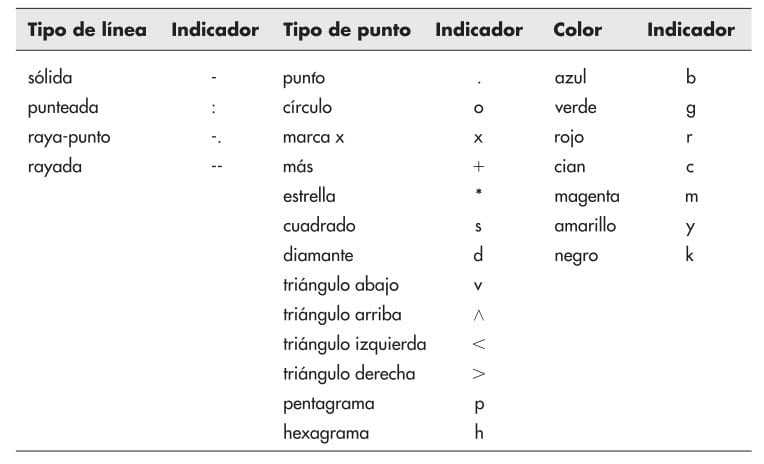
\includegraphics[width = 100mm]{imagenes/atributos-MATLAB}
		\label{estilos}
		\caption{Estilos y colores en gráficas}
	\end{figure}

	\item Para ello se pone \textcolor{green}{plot(a,b,'atributos')}
	
	\item Para cambiar el tamaño de la línea se utiliza el comando \textcolor{green}{linewigth} y para el tamaño de la fuente \textcolor{green}{FontSize}. Para cambiar la fuente de los Axes se usa el comando \textcolor{green}{gca}.
	
	\item \textcolor{green}{plot(a,b,'atributos','linewitdh',6)}
	
	\item \textcolor{green}{title('Función de Seno','FontSize',15)}
	
	\item \textcolor{green}{set(gca,'fontsize',14)}
	\subsection{Escalamiento de Ejes}
	
	\item Se utilizan los comandos \textcolor{blue}{axis([xmin xmax ymin ymax])}
	
	\item Para crear anotaciones dentro de la gráfica se utiliza el comando \textcolor{blue}{text(Posición en $x$, Posición en $y$, 'Leyenda')}
	
	\item Para controlar más sobre los parámetros de plot, utilizar el comando \textcolor{blue}{help plot}
	
	\end{itemize}


	\section{Episodio 17: Animaciones en Gráficas MatLab}
	
	Para ello se utiliza la interfaz interna del programa GUIDE. Los pasos para ello son los siguientes:
	
	\begin{itemize}
		\item Crear una figura: Este es el espacio de trabajo del programa; Para ello se porsigue asi: 
		
		\textcolor{violet}{fig(1)=figure('name', 'Monitor','menubar','none','position',[200 200 800 700],'color',[0.9 0.6 0.3])}
		
	\item Para crear los Axes:
		
		\textcolor{violet}{axe(1)=axes('parent',fig(1),'units','pixels','position',[60 80 600 550],'xlim',[0 40].'ylim',[-3 3],'xgrid','on','ygrid','on')}
		
	\item Para el nombre de los ejes:
	
	\textcolor{violet}{set(get(axe(1),'Xlabel'),'String','Tiempo (Seg)')}
	
	\textcolor{violet}{set(get(axe(1),'Ylabel'),'String','Función')}
	
	\item Para la creación de los atributos de las líneas:
	
	\textcolor{violet}{lin(1)=Line('parent','axe(1)','xdata',[ ],'ydata',[ ],'Color','r','LineWidth', 2.5)}
	
	\textcolor{violet}{lin(2)=Line('parent','axe(1)','xdata',[ ],'ydata',[ ],'Color','k','LineWidth', 2)}
	
	
	\begin{figure}[h!]
		\centering
		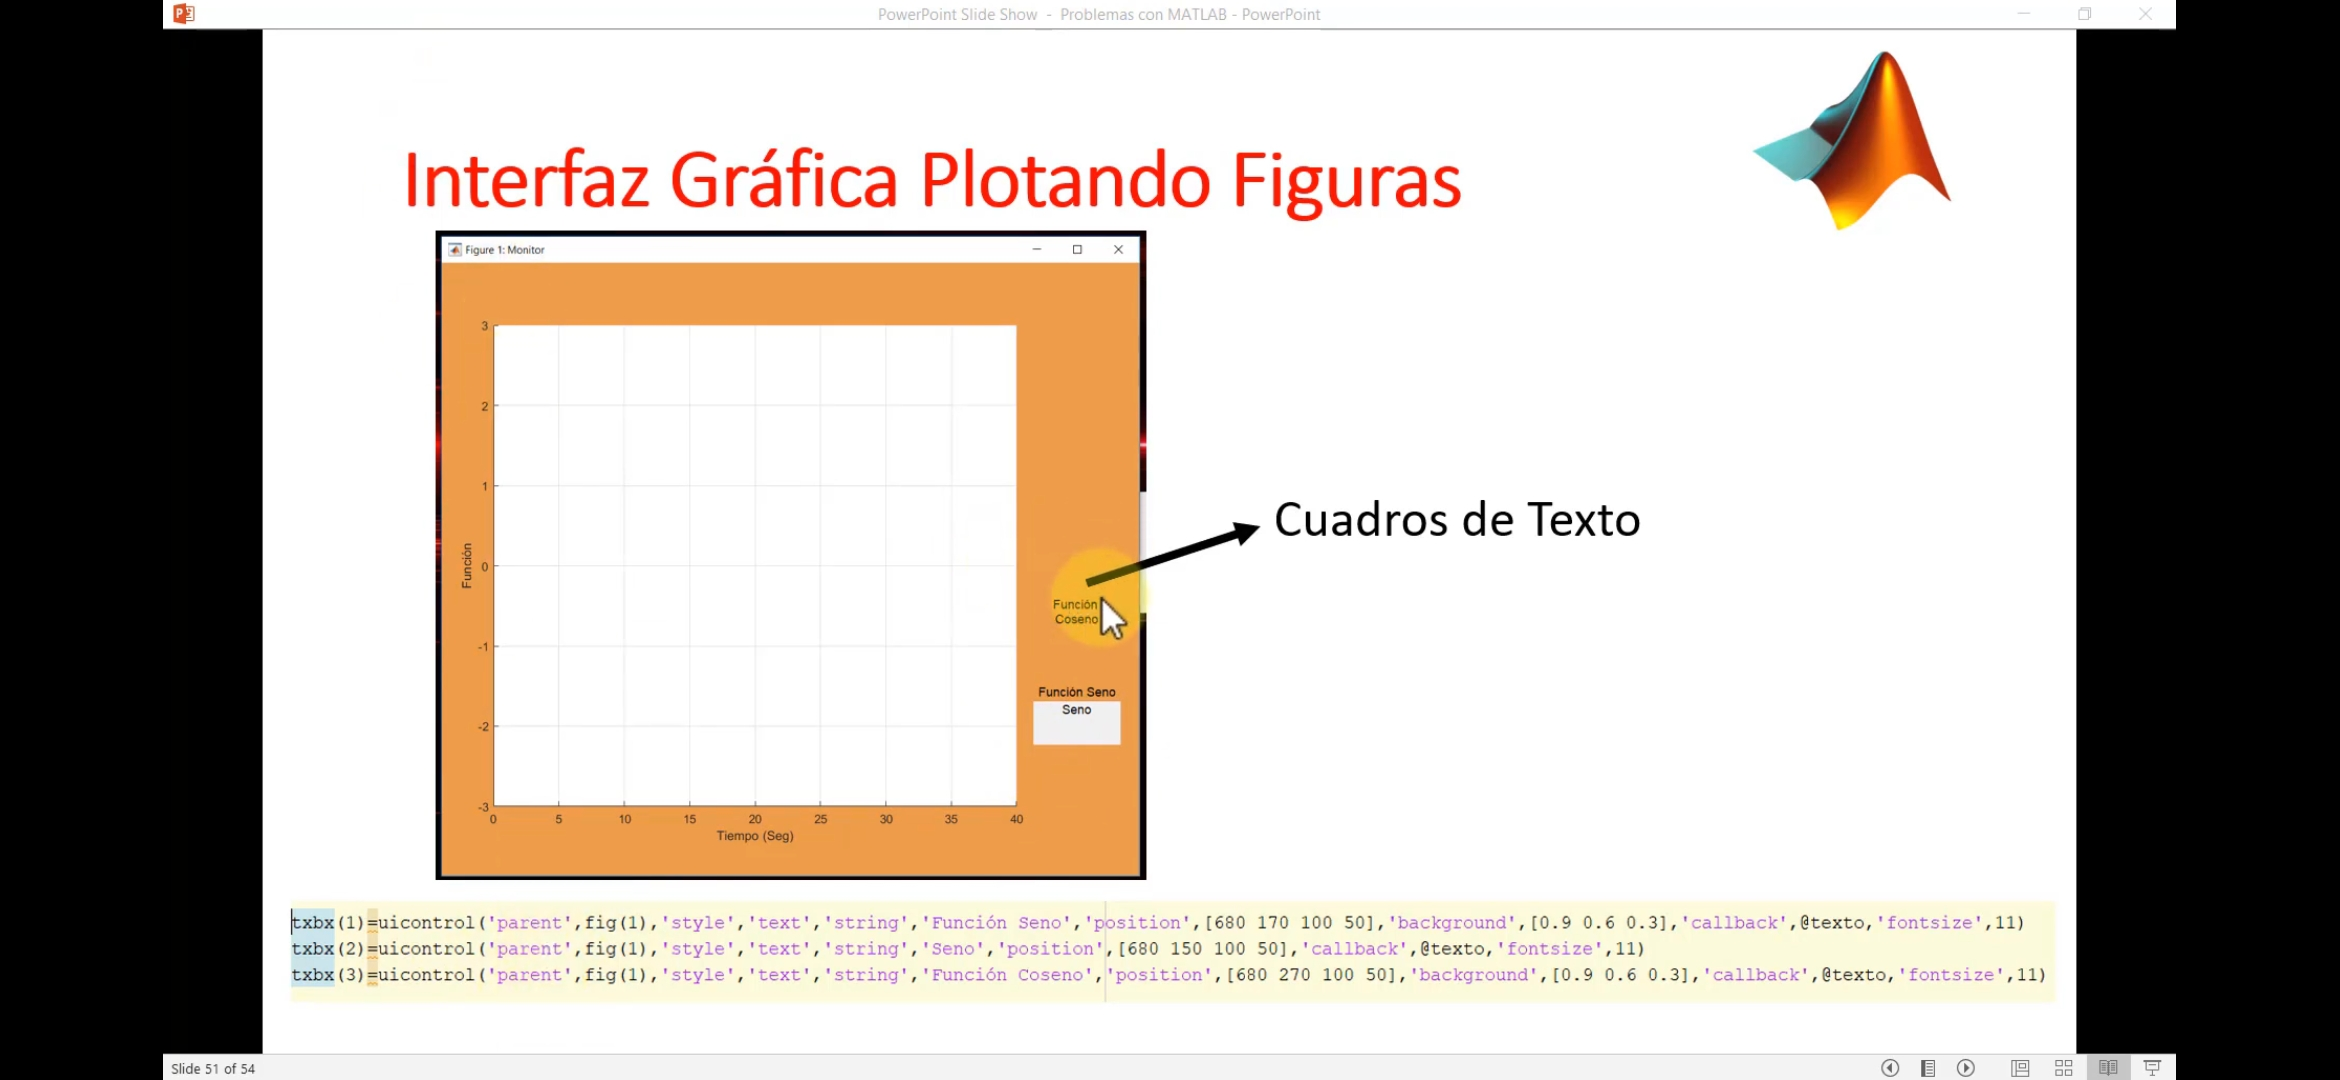
\includegraphics[width = 100mm]{imagenes/Funciones/1}
		\label{txt}
		\caption{Cuadro de texto}
	\end{figure}


	\begin{figure}[h!]
		\centering
		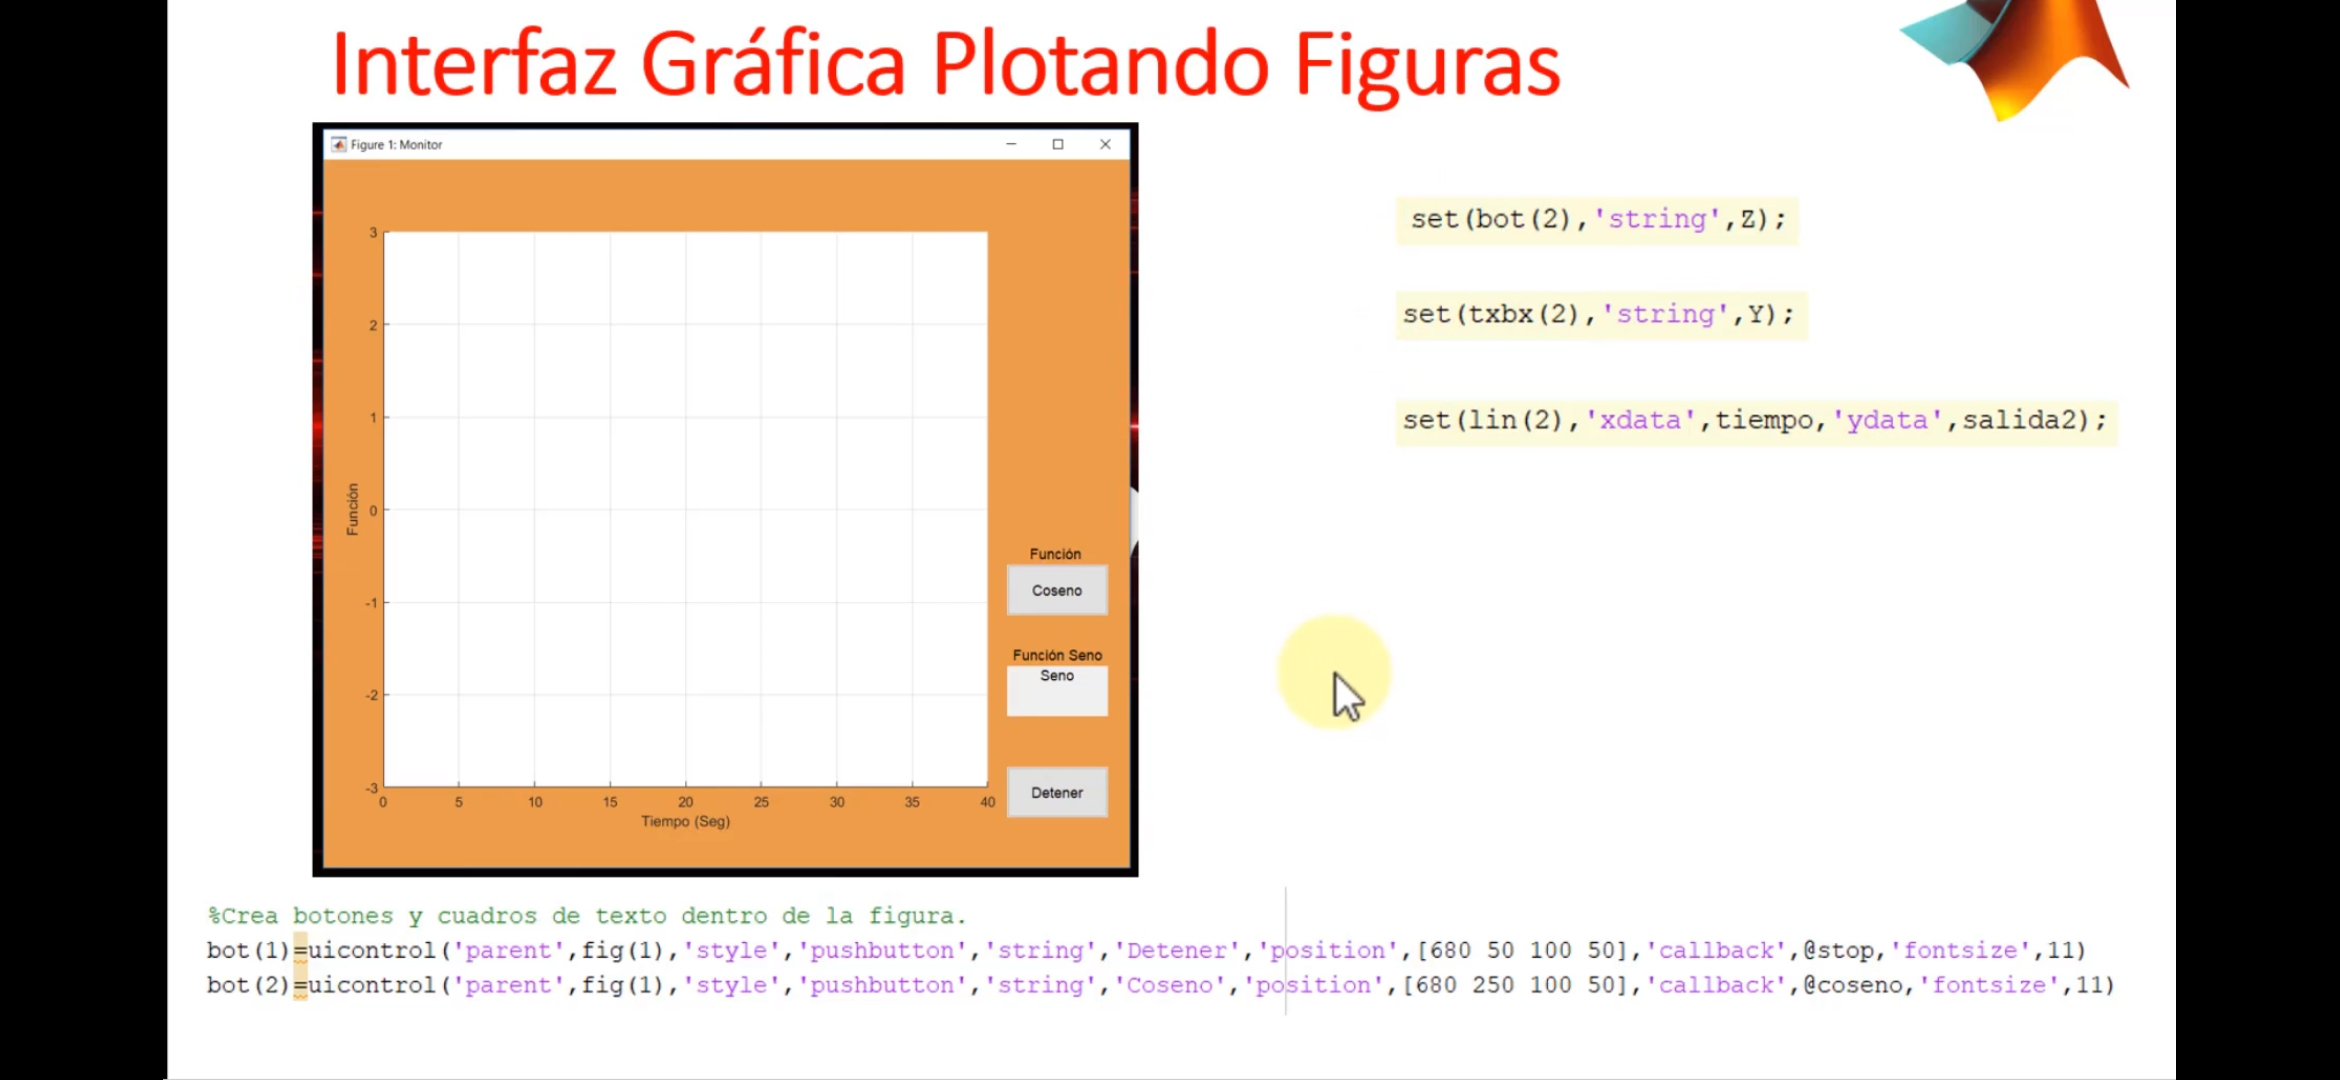
\includegraphics[width = 100mm]{imagenes/Funciones/6}
		\label{botones}
		\caption{Botones}
	\end{figure}


	\begin{figure}[h!]
		\centering
		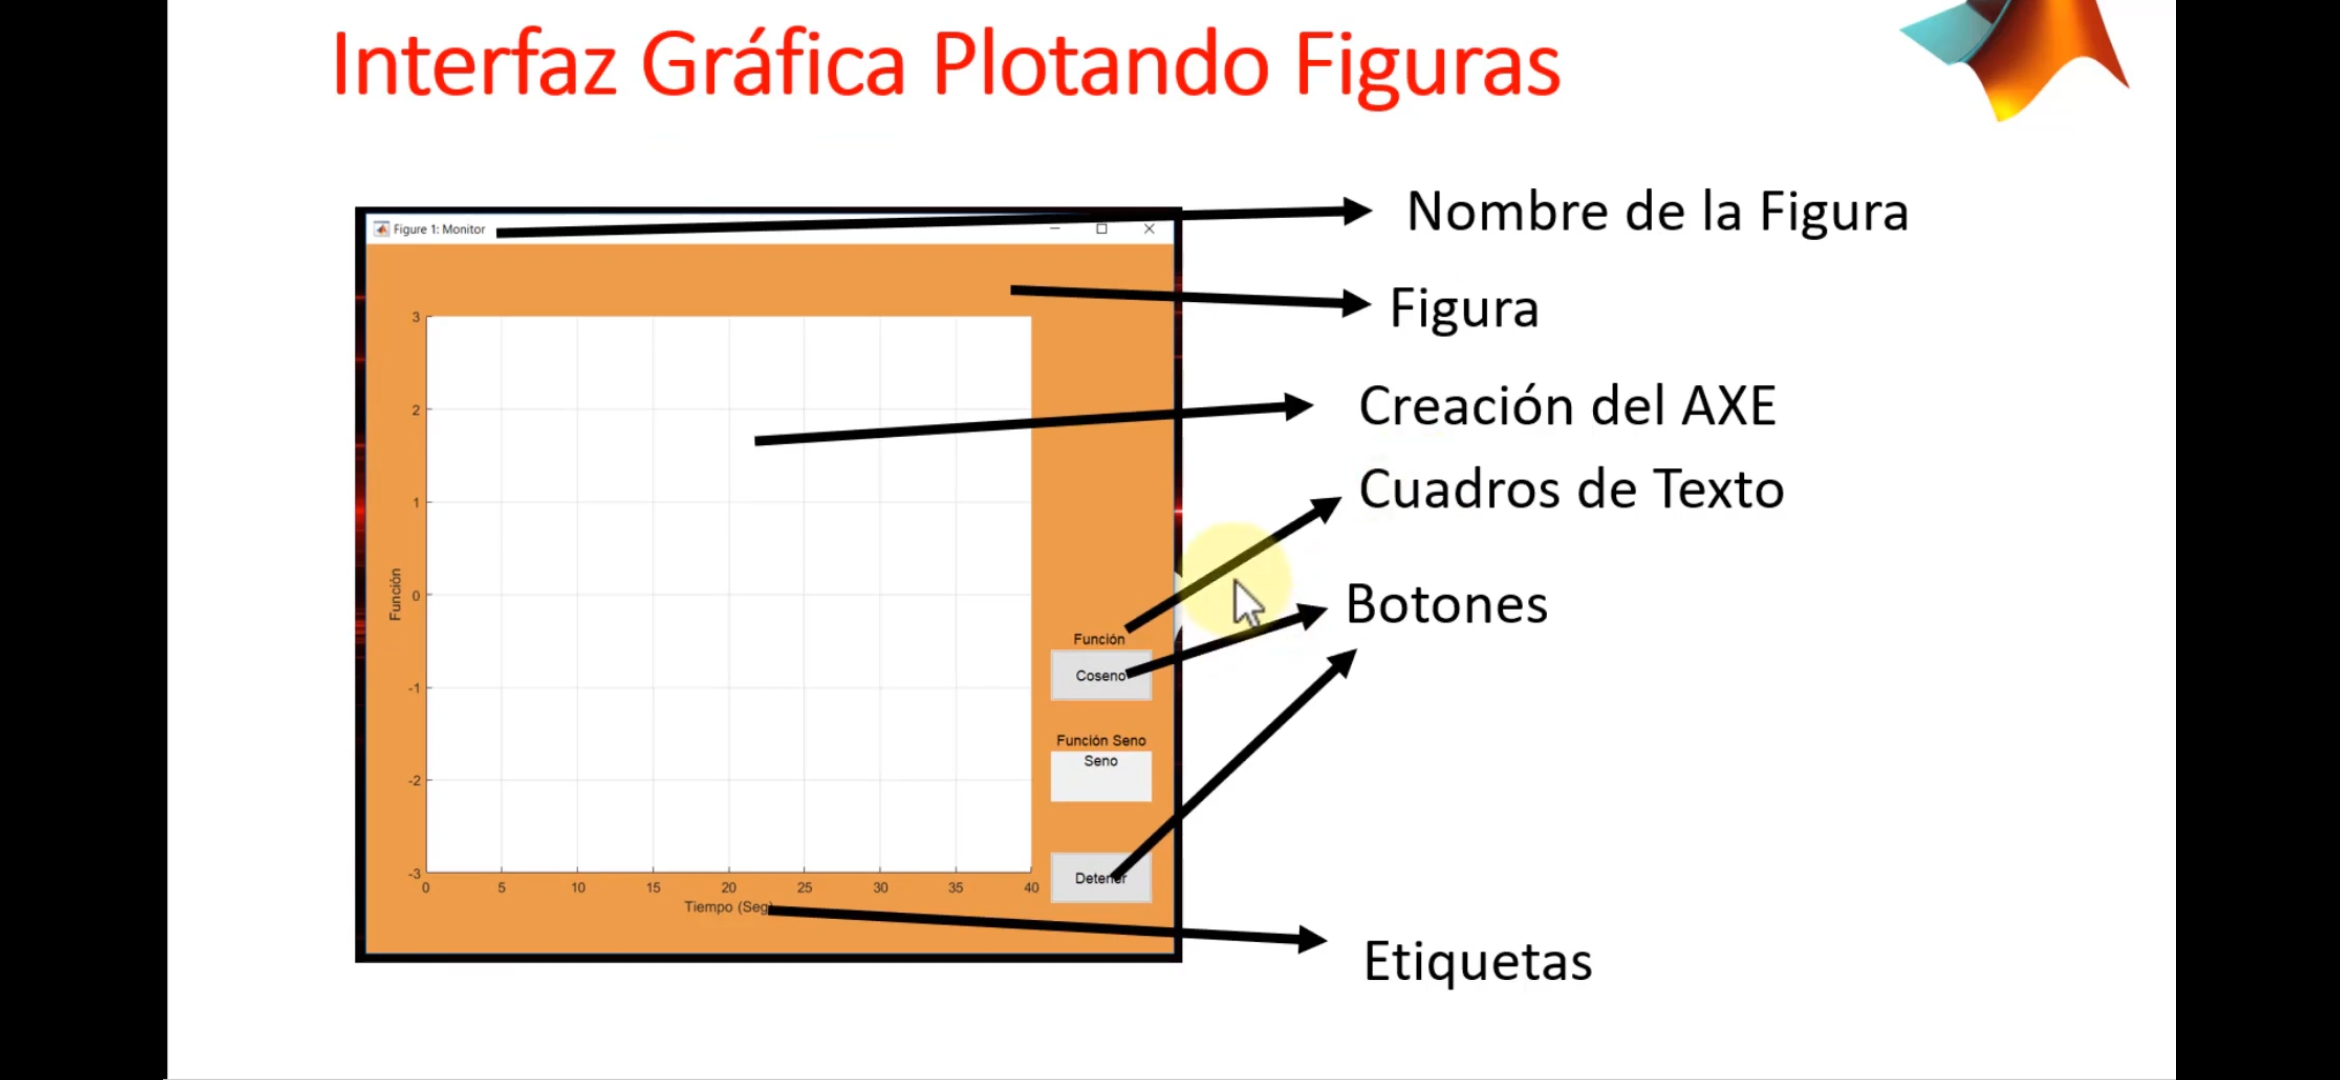
\includegraphics[width = 100mm]{imagenes/Funciones/8}
		\label{final}
		\caption{Interfaz final}
	\end{figure}
	
	VER EPISODIO COMPLETO 

	
	\section{Episodio 18: Gráficas Polares en MatLab}
	
	Las otras formas de representar los datos son:
	
	\begin{itemize}
		\item La función \textcolor{purple}{polar(theta,r)} con el ángulo theta en radianes
		
		Ejemplo 1:
		
		figure
		
		x=0:pi/100:pi;
		
		y = sin(x);
		
		polar(x,y)
		
		\item Flor:
				
		figure
		
		theta = 0:0.01*pi:2*pi;
		
		r = 5*cos(4*theta);
		
		polar(theta,r)
		
		\item Estrella
				
		figure
		
		theta = pi/2:4/5*pi:4.8*pi;
		
		r=ones(1,6);
		
		polar(theta,r)
	\end{itemize}
	
	
	\end{itemize}


	\section{Episodio 19: Arreglo de Gráficas}
	
				
	Para emplear las gráficas logaritmicas se ultiliza de la siguiente manera:
	
	\begin{figure}[h!]
		\centering
		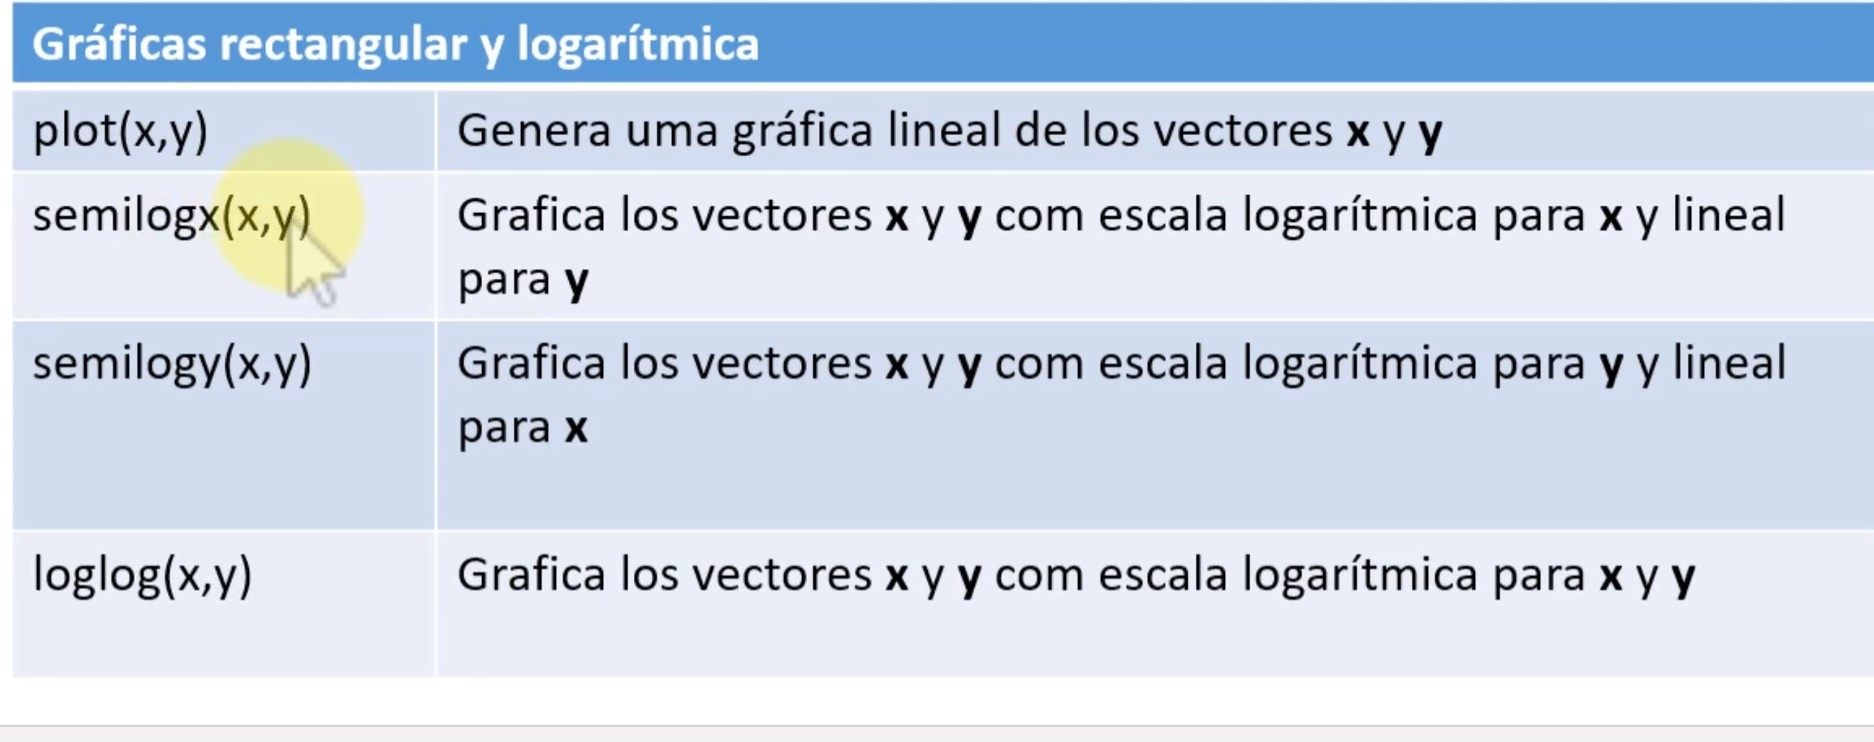
\includegraphics[width = 100mm]{imagenes/Funciones/logaritmica}
		\label{logarit}
		\caption{Arreglo logarítmico para gráficas}
	\end{figure}
				
	\begin{itemize}
		\item Ejemplo: Graficar $y = 5x^2$ con los cuatro enfoques de escalamiento
		
		$x = 0:0.5:50;$		[Vector de x]
		
		$y = 5*x.^2;$		[Función de y (El punto es importante para que eleve cada elemento del vector al cuadrado)]
		
		subplot(2,2,1) \\
		plot(x,y)\\
		title('Polinomial-Lineal-lineal')\\
		ylabel('y'), grid
		
		subplot(2,2,2) \\
		semilogx(x,y)\\
		title('Polinomial-Logaritmica-Lineal')\\
		ylabel('y'), grid
		
		subplot(2,2,3) \\
		semilogy(x,y)\\
		title('Polinomial-Lineal-Logaritmica')\\
		xlabel('x'), grid
		
		subplot(2,2,4) \\
		loglog(x,y)\\
		title('Polinomial-Logaritmica- Logaritmica')\\
		xlabel('x'), grid
		
	\end{itemize}	
		
	\section{Episodio 20: Gráfica de Barras y Pastar en MatLab}
	
	Los diferentes tipos de gráficos disponibles son:
	
	\begin{figure}[h!]
		\centering
		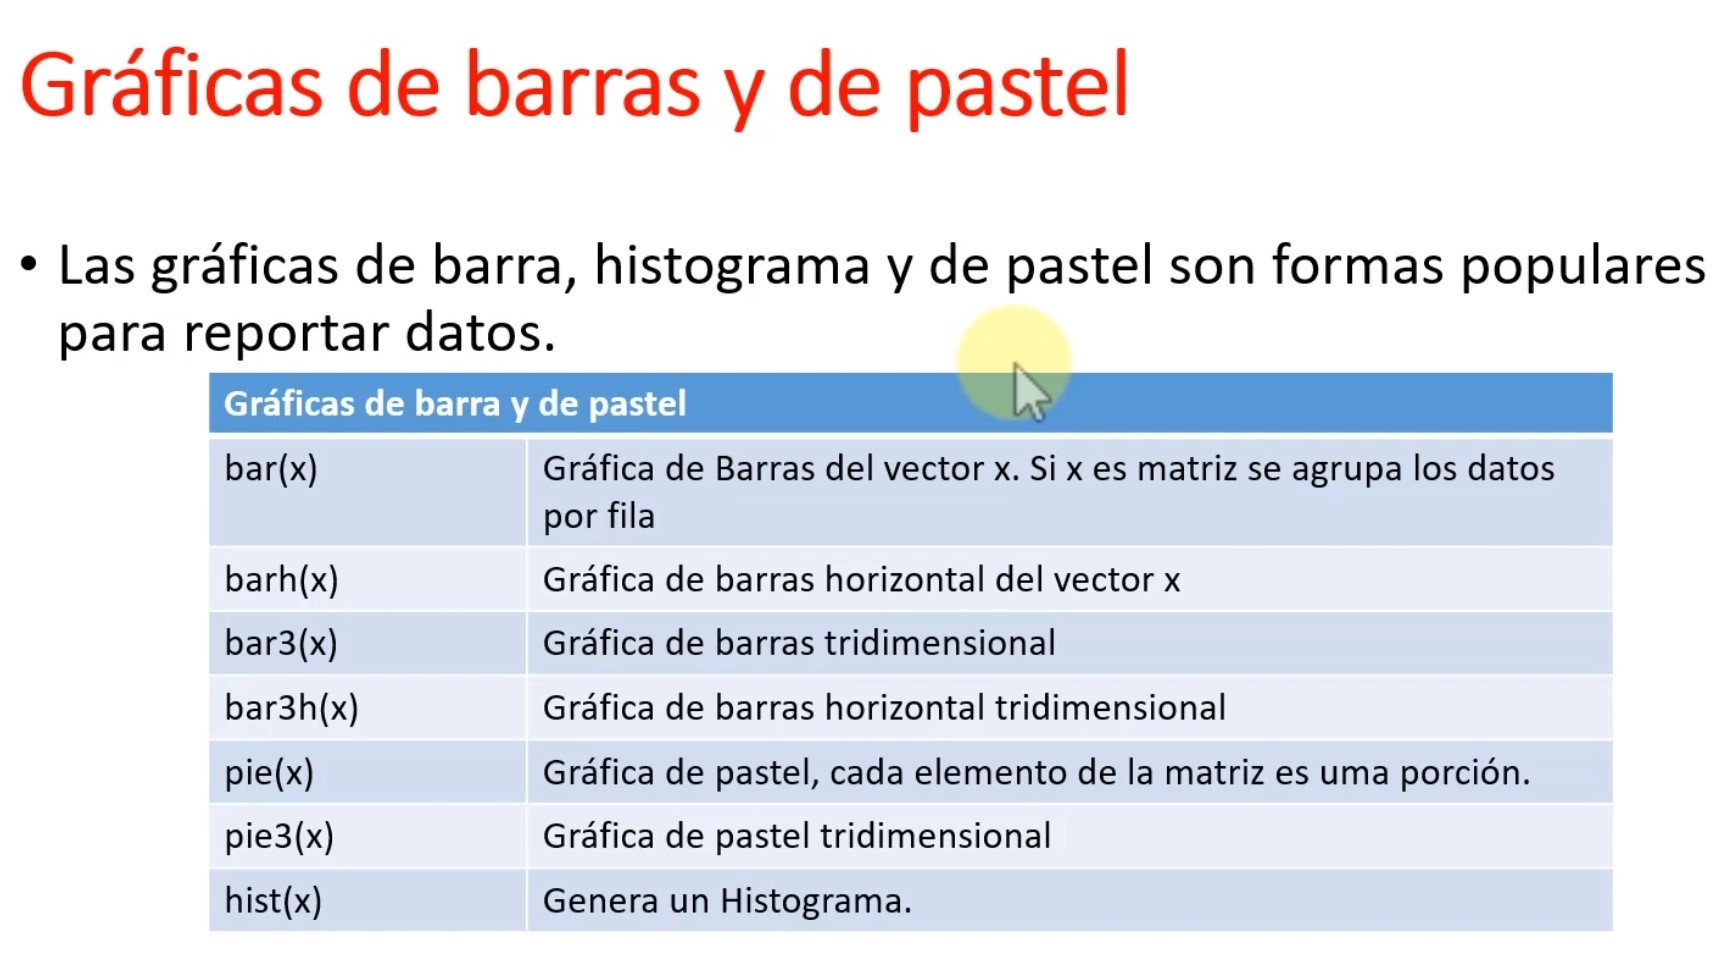
\includegraphics[width = 100mm]{imagenes/Funciones/barras}
		\label{barras}
		\caption{Tipos de gráficas}
	\end{figure}

	\begin{itemize}
		\item Ejemplo 1:
		
		x = [1 2 5 4 8];
		y = [x;1:5]
		
		figure\\
		subplot(2,2,1)\\
		bar(x)\\
		title('Gráfica de Barras del vector $x$')
		
		subplot(2,2,2)\\
		bar(y)\\
		title('Gráfica de la matriz $y$')
		
		subplot(2,2,3)\\
		bar3(x)\\
		title('Gráfica tridimensional de Barras del vector $x$')
		
		subplot(2,2,4)\\
		bar3h(y)\\
		title('Gráfica tridimensional de Barras Horizontales de la matriz $y$')
		
	\end{itemize}
	
	\section{Episodio 21: Histograma}
	
	Para hacer un histograma, el defecto son 10 depósitos o categorías.
	
	\begin{itemize}
		\item Ejemplo 1: Calificaciones de alumnos
		
	El comando a utilizar es \textcolor{green}{hist(x,n)} donde $n$ es el número de depósitos. También se puede almacenar el histograma en una variable \textcolor{green}{A = hist(x,n)}
	
	\textcolor{purple}{hist help} recomienda usar en vez \textcolor{purple}{HISTOGRAM}
	\end{itemize}

	\section{Episodio 22: Graficar en MatLab en 3D}
	
	MatLab utiliza los siguientes comandos para graficar:
	
		\begin{figure}[h!]
		\centering
		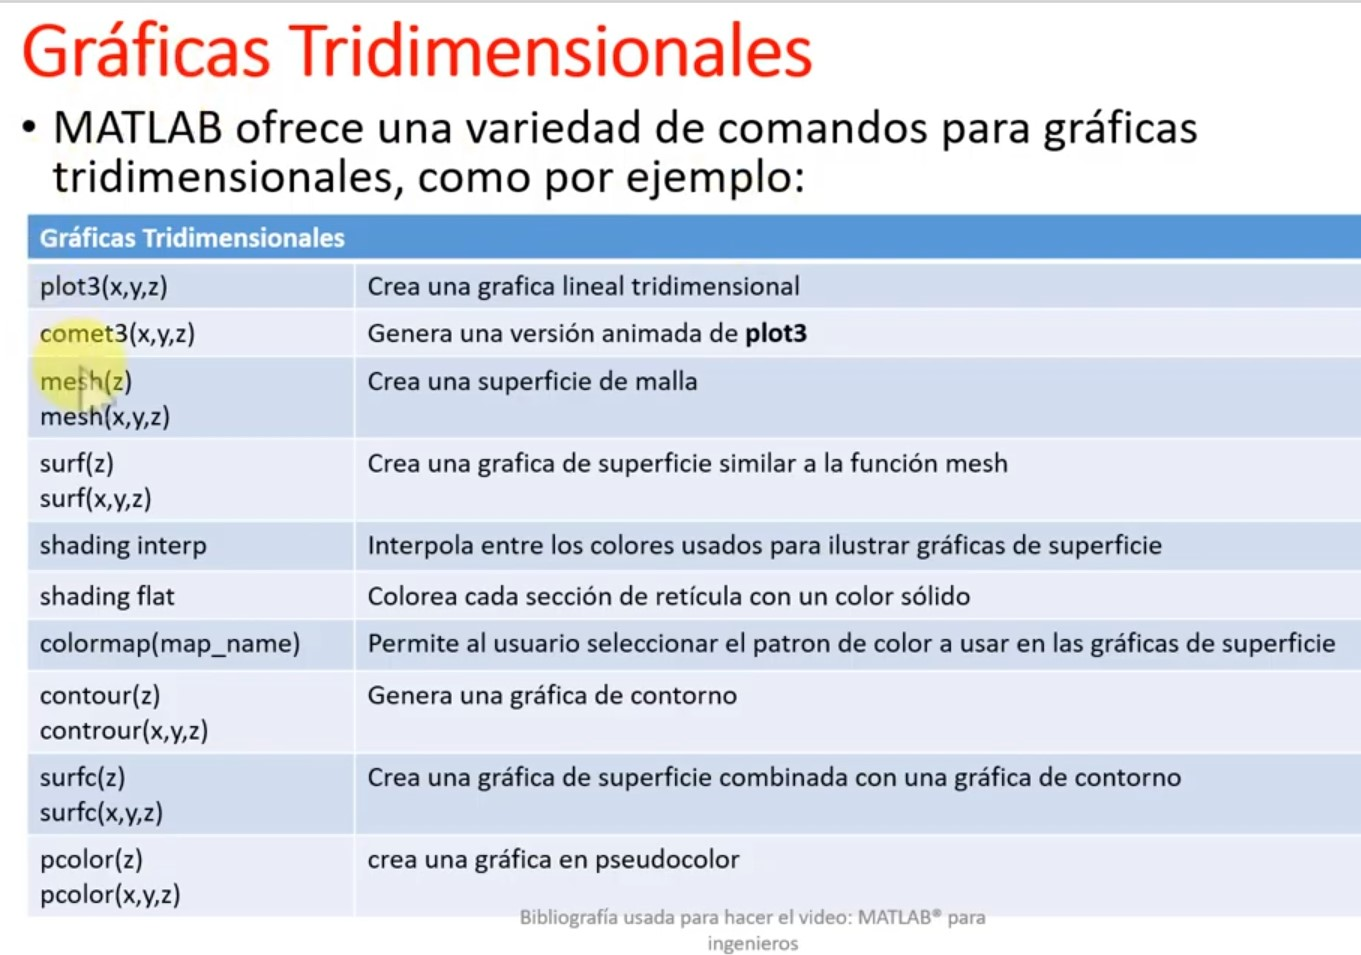
\includegraphics[width = 100mm]{imagenes/Funciones/graficas3d}
		\label{3d}
		\caption{Tipos de gráficas en 3D}
	\end{figure}
	
	\section{Episodio 23: Superficie en Gráficas 3D}
	
	\begin{itemize}
		\item Las gráficas Mesh son muy utilizadas en procesos de optimización de ingeniería
		\item La función Surf crea una superficie tridimensional en vez de un mallado, para controlar las sombras se utiliza el comando \textcolor{purple}{shading + opción}
	\end{itemize}

	\section{Episodio 24: Gráficas de Contorno y Superficie}

	\begin{itemize}
		\item El comando \textcolor{purple}{[X,Y] = meshgrid(x,y)} se utiliza para crear una grilla
		\item La función \textcolor{purple}{sufc} combina la gráfica de superficie con la gráfica de contorno
	\end{itemize}
		
	\begin{figure}[h!]
		\centering
		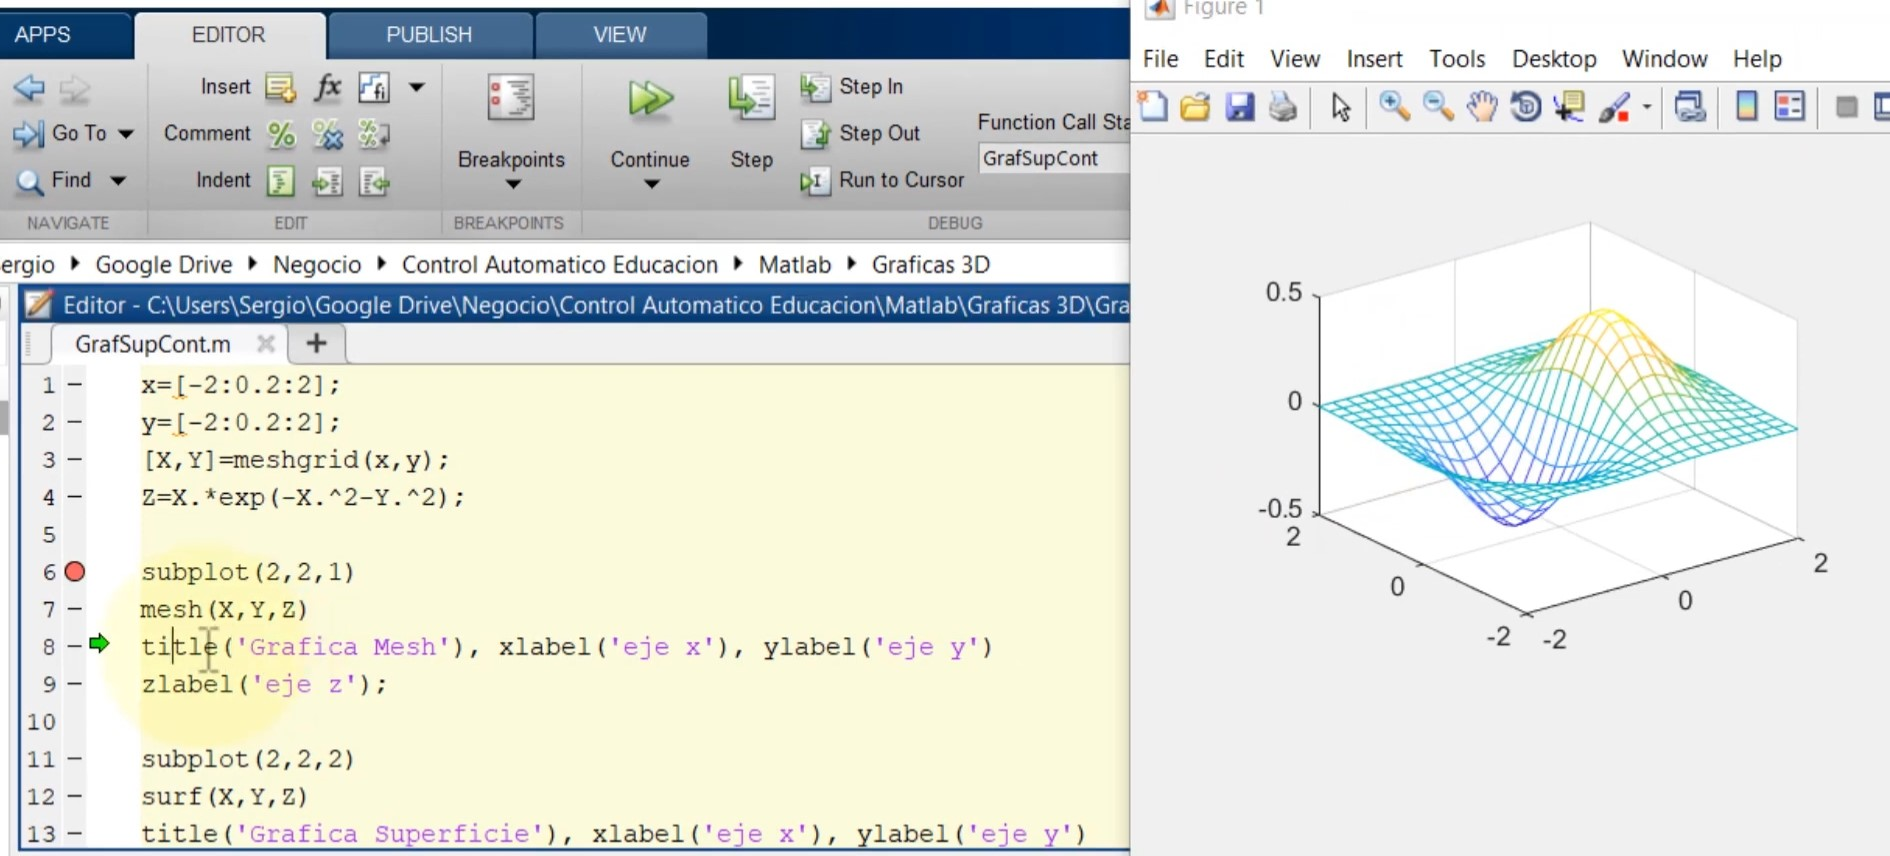
\includegraphics[width = 100mm]{imagenes/Funciones/ejemplodemeshgrid}
		\label{gridejemplo}
		\caption{Ejemplo del comando meshgrid}
	\end{figure}
	
	\begin{itemize}
		\item Para utilizar el colormap 
	\end{itemize}

		\begin{figure}[h!]
		\centering
		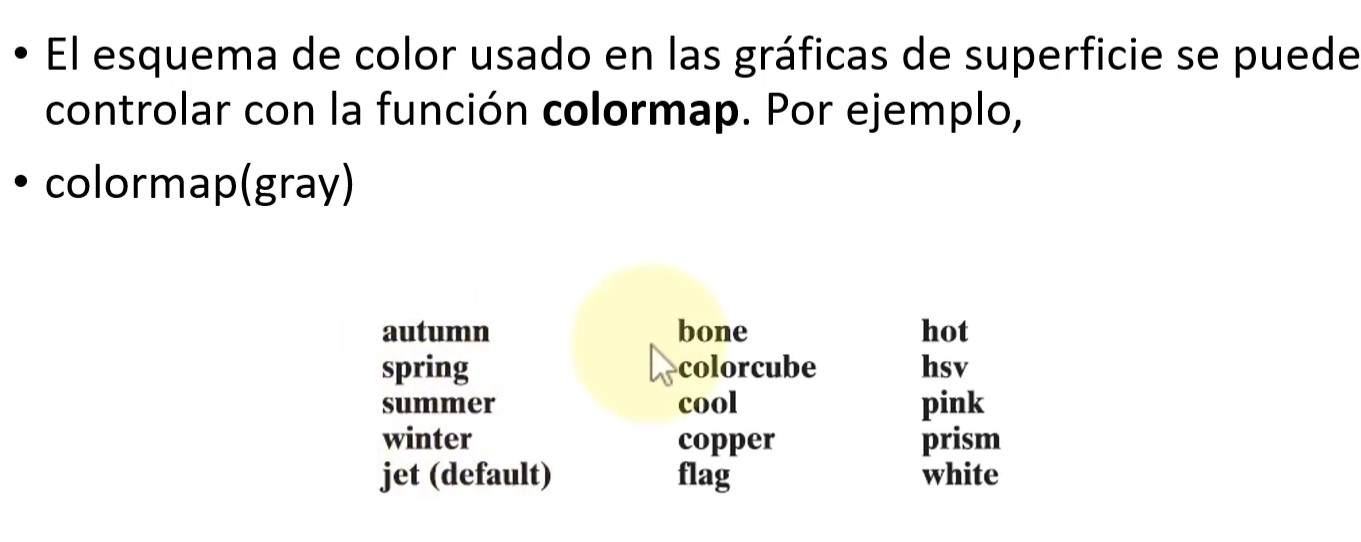
\includegraphics[width = 100mm]{imagenes/Funciones/colormap}
		\label{colormap}
		\caption{Ejemplos del colormap}
	\end{figure}
	
	\begin{itemize}
		\item En el comando \textcolor{purple}{pcolor} para quitar la cuadricula se utiliza el comando \textcolor{green}{shading interp}
	\end{itemize}
	
	
\end{document}